\documentclass[12pt]{report}

% Packages
% ========
\usepackage[letterpaper, portrait, margin=1in]{geometry}
\usepackage{graphicx}			% So we can load figures with "." in their filename
\usepackage{float}				% So we can use "[H]"
\usepackage[dvipsnames]{xcolor}	% For custom colors
\usepackage{xparse}				% For \DeclareDocumentCommand
\usepackage{caption}			% For \captionof command
\usepackage{mathtools}			% For \DeclarePairedDelimeter
\usepackage{ifthen}				% For \ifthenelse{}{}{}
\usepackage{soul}				% For underlining with \ul
\setuldepth{x}					%	""
\usepackage{multicol}			% For multiple columns via \begin{multicols}{2}
\usepackage[most]{tcolorbox}	% For the tl; dr environment
\usepackage{array}				% For extended column definitions
\usepackage{tabularray}			% For \begin{longtblr} tables that span multiple columns and pages
\usepackage{amssymb}			% For $\checkmark$
\usepackage{etoc}				% For \localtableofcontents


% Inserting code into LaTeX: \begin{lstlisting} ...
\usepackage{listings}
\definecolor{dkgreen}{rgb}{0,0.6,0}
\definecolor{gray}{rgb}{0.5,0.5,0.5}
\definecolor{mauve}{rgb}{0.58,0,0.82}

\lstset{frame=tb,
  language=C++,
  aboveskip=3mm,
  belowskip=3mm,
  showstringspaces=false,
  columns=flexible,
  basicstyle={\small\ttfamily},
  numbers=none,
  numberstyle=\tiny\color{gray},
  keywordstyle=\color{blue},
  commentstyle=\color{dkgreen},
  stringstyle=\color{mauve},
  breaklines=true,
  breakatwhitespace=true,
  tabsize=3
}

% Inline code
\definecolor{darkpink}{rgb}{0.5, 0.0, 0.5}
\newcommand{\code}[1]{\texttt{\color{darkpink}#1}}

% Bibliography
% ============
\usepackage[american]{babel}
\usepackage{csquotes}
\usepackage[style=ieee, backend=biber]{biblatex}
\usepackage{hyperref}
\hypersetup{colorlinks=true, allcolors=black, urlcolor=blue}
\addbibresource{../sources.bib}

% etoc setup
% ==========

\etocsetstyle{section}{}{}{\etocsavedchaptertocline{\numberline{}\etocname}{\etocpage}}{}
\etocsetstyle{subsection}{}{}{\etocsavedsectiontocline{\numberline{}\etocname}{\etocpage}}{}
\etocsetstyle{subsubsection}{}{}{\etocsavedsubsectiontocline{\numberline{}\etocname}{\etocpage}}{}
\etocsetstyle{paragraph}{}{}{\etocsavedsubsubsectiontocline{\numberline{}\etocname}{\etocpage}}{}
\etocsetstyle{subparagraph}{}{}{\etocsavedparagraphtocline{\numberline{}\etocname}{\etocpage}}{}


% Simple custom commands
% ======================
\makeatletter
\def\maxwidth#1{\ifdim\Gin@nat@width>#1 #1\else\Gin@nat@width\fi} 
\makeatother

\def\todo#1{\selectfont{\color{red}\texttt{\textbf{TODO:} #1}}}

% Sections 'n' such
% =================

\definecolor{chaptColor}{RGB}{0, 83, 161}

\def\chapt#1{
%
	% Default chapter behavior
	\begingroup\color{chaptColor}
	\chapter{#1}
	\endgroup
	
	% Label
	\label{chp:#1}
}

\definecolor{sectColor}{rgb}{0, 0.5, 0.0}
\def\sect#1{\textcolor{sectColor}{\section{#1}}}

\definecolor{subsectColor}{rgb}{0, 0.5, 0.5}
\def\subsect#1{\textcolor{subsectColor}{\subsection{#1}}\noindent}

\definecolor{subsubsectColor}{rgb}{0.747, 0.458, 0}
\def\subsubsect#1{\textcolor{subsubsectColor}{\subsubsection{#1}}}

% TL; DR section
% ==============
\newenvironment{tldr}{\begin{tcolorbox}[colback=gray!20!white,colframe=blue!75!black,title=TL; DR]}{\end{tcolorbox}\vspace*{12pt}}

% Custom math commands
% ====================
\DeclarePairedDelimiter\ceil{\lceil}{\rceil}
\DeclarePairedDelimiter\floor{\lfloor}{\rfloor}

% ======================
% \graphic{filename=...}
% ======================
% Keyword arguments
\makeatletter
\define@key{graphicKeys}{filename}{\def\graphic@filename{#1}}
\define@key{graphicKeys}{scale}{\def\graphic@scale{#1}}
\define@key{graphicKeys}{width}{\def\graphic@width{#1}}
\define@key{graphicKeys}{caption}{\def\graphic@caption{#1}}
\define@key{graphicKeys}{captionType}{\def\graphic@captionType{#1}}
\define@key{graphicKeys}{label}{\def\graphic@label{#1}}

% Kwargs
\DeclareDocumentCommand{\graphic}{m}{

	\begingroup
	
	% Set default kwargs
	\setkeys{graphicKeys}{filename={0}, #1}
	\setkeys{graphicKeys}{scale={0}, #1}
	\setkeys{graphicKeys}{width={0}, #1}
	\setkeys{graphicKeys}{caption={}, #1}
	\setkeys{graphicKeys}{captionType={figure}, #1}
	\setkeys{graphicKeys}{label={}, #1}
	
	% Assign width
	\let\graphicWidth\relax % let \mytmplen to \relax
	\newlength{\graphicWidth}
	\setlength{\graphicWidth}{\columnwidth}
	
	\if \graphic@scale 0
		
		\if \graphic@width 0
			
			\setlength{\graphicWidth}{0.5\columnwidth}
		
		\else
	
			\setlength{\graphicWidth}{\graphic@width}
			
		\fi

	\else
		
		\setlength{\graphicWidth}{\columnwidth * \graphic@scale}

	\fi	
	
	% Do figure
	\begin{minipage}{\columnwidth}
		\vspace*{12pt}
		\begin{center}
		
			\includegraphics[width = \graphicWidth]{\graphic@filename}
			
			\ifthenelse{\equal{\graphic@caption}{}}{}{
				\captionof{\graphic@captionType}{\graphic@caption}
			}
			
			\ifthenelse{\equal{\graphic@label}{}}{
				\label{fig: \graphic@filename}
			}{
				\label{\graphic@label}
			}
		\end{center}
		\vspace*{12pt}
	\end{minipage}
	
	\endgroup
}
\makeatother

% ==============
% Base Pair Page
% ==============
% Keyword arguments
\makeatletter
\define@key{bpPageKeys}{baseFilename}{\def\bpPage@baseFilename{#1}}
\define@key{bpPageKeys}{scale}{\def\bpPage@scale{#1}}
\define@key{bpPageKeys}{width}{\def\bpPage@width{#1}}
\define@key{bpPageKeys}{caption}{\def\bpPage@caption{#1}}
\define@key{bpPageKeys}{captionType}{\def\bpPage@captionType{#1}}
\define@key{bpPageKeys}{label}{\def\bpPage@label{#1}}

% Kwargs
\DeclareDocumentCommand{\BPPage}{m}{

	\begingroup
	
	% Set default kwargs
	\setkeys{bpPageKeys}{baseFilename={0}, #1}
	\setkeys{bpPageKeys}{caption={}, #1}
	\setkeys{bpPageKeys}{label={}, #1}
	
	\newpage

	\begin{center}
		\ul{\mbox{\bpPage@baseFilename{}: 1 Base Pair [min]}}
	\end{center}
	\vspace*{-36pt}
	\begin{minipage}[b]{0.5\textwidth}
		\graphic{filename=\bpPage@baseFilename-overview-1-table, width=\textwidth}
	\end{minipage}
	\begin{minipage}[b]{0.5\textwidth}
		\graphic{filename=\bpPage@baseFilename-overview-1-plot, width=\textwidth}
	\end{minipage}

	\begin{center}
		\ul{\mbox{\bpPage@baseFilename{}: 50 Base Pairs [average]}}
	\end{center}
	\vspace*{-36pt}
	\begin{minipage}[b]{0.5\textwidth}
		\graphic{filename=\bpPage@baseFilename-overview-50-table, width=\textwidth}
	\end{minipage}
	\begin{minipage}[b]{0.5\textwidth}
		\graphic{filename=\bpPage@baseFilename-overview-50-plot, width=\textwidth}
	\end{minipage}
	
	\begin{center}
		\ul{\mbox{\bpPage@baseFilename{}: 100 Base Pairs [max]}}
	\end{center}
	\vspace*{-36pt}
	\begin{minipage}[b]{0.5\textwidth}
		\graphic{filename=\bpPage@baseFilename-overview-100-table, width=\textwidth}
	\end{minipage}
	\begin{minipage}[b]{0.5\textwidth}
		\graphic{filename=\bpPage@baseFilename-overview-100-plot, width=\textwidth}
	\end{minipage}

	\vspace*{-24pt}
	\captionof{figure}{\bpPage@caption}\label{\bpPage@label}	
	
	\endgroup
}
\makeatother



\begin{document}

\begin{tldr}
	\todo{}
\end{tldr}

\sect{Structure}

\newcommand{\SubItem}[1]{\begin{itemize}\item{#1}\end{itemize}}

\begin{itemize}
	\item{\textbf{\code{EffectableComponent}s} are \code{ActorComponent}s that allow for delegation (effects). They have predefined places that allow for code modification. 
		\SubItem{Let's use \code{StatsComponent} as an example. Say we want a Pok\'{e}mon-style ``Adamant'' nature ($+$10\% PhA/$-$10\%SpA). One such place for modification is in the function \code{RecalculateStats}.}
		\begin{center}
			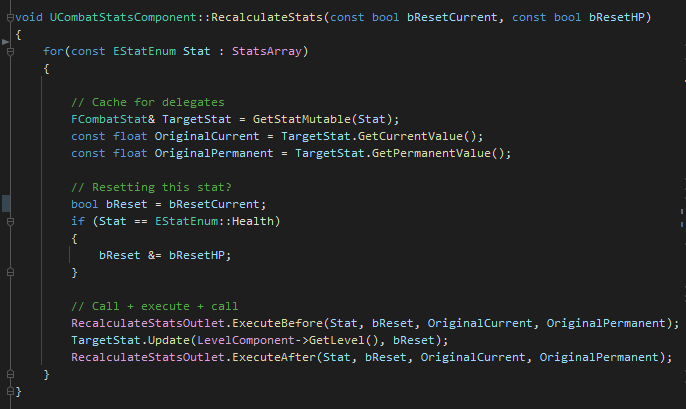
\includegraphics[scale=2.5]{recalculate-stats-code}
		\end{center}
		}
	\item{\textbf{Delegate arrays} are variables inside of \code{EffectableComponent}s. They hold functions that execute when needed.
		\SubItem{Let's use \code{StatsComponent}'s \code{AfterRecalculateStatsArray} in our example. In this case, after stats are recalculated (say, on level-up), the base PhA would increase by 10\% and the base SpA would decrease by 10\% (additively): }
		\begin{center}
			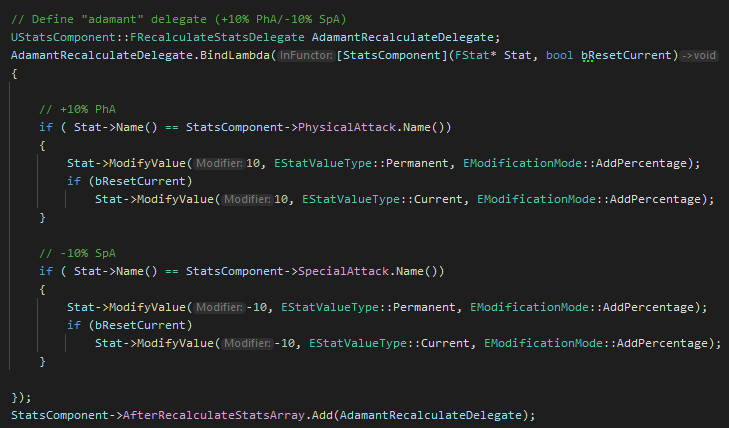
\includegraphics[scale=2.5]{adamant-code}
		\end{center}		 
		}
\end{itemize}

\sect{List of \code{EffectableComponent}s and Delegate Arrays}

The following tables show all implemented \code{EffectableComponent}s and their delegate arrays. Note the ``base name'' indicates existence of:

\begin{enumerate}
	\item{the delegate type \code{FBaseNameDelegate};}
	\item{the before/after arrays of delegates: \\\code{TArray<FBaseNameDelegate> BeforeBaseNameArray}; and}
	\item{a function for each before/after to execute the arrays: \code{ExecuteBeforeBaseName (...)}.}
\end{enumerate}

\noindent Note that the philosophy applies to what is \textit{probable} rather than what is \textit{possible}. Hence the list meant to be practical rather than exhaustive.

\begin{longtblr}[
	caption = {Delegate Arrays for \code{AffinitiesComponent}},
	label = {delegate-arrays-affinitiescomponent},
]{
	colspec= {Q[r, wd=0.25\linewidth] Q[l, wd=0.35\linewidth] Q[l, wd=0.25\linewidth]},
	hline{1,Z} = {2pt},
	hlines,
	row{1} = {font=\bfseries},
}

	Delegate Array Base Name	& Parameters	& Note\\
	GetUnspentPoints			& \code{int\&} Unspent points\\
	SetUnpentPoints				& \code{int\&} Current unspent points\\
								& \code{int\&} Attempted value being set\\
	
\end{longtblr}

\begin{longtblr}[
	caption = {Delegate Arrays for \code{LevelComponent}},
	label = {delegate-arrays-levelcomponent},
]{
	colspec= {Q[r, wd=0.25\linewidth] Q[l, wd=0.35\linewidth] Q[l, wd=0.25\linewidth]},
	hline{1,Z} = {2pt},
	hlines,
	row{1} = {font=\bfseries},
}

	Delegate Array Base Name	& Parameters	& Note\\
	GetBaseExpYield				& \code{int} Unaltered base exp yield\\
	SetBaseExpYield				& \code{int} Unaltered base exp yield\\
								& \code{int\&} Attempted value being set\\
	GetExpYield					& \code{UStatsComponent*} Victorious Monster\\
								& \code{float\&} Awarded exp\\
	GetCumulativeExp			& \code{int\&} Current CXP\\
	SetCumulativeExp			& \code{int} Current CXP	& All other level/exp setters go through here!\\
								& \code{int\&} Attempted CXP\\
	AddExp						& \code{int} Current exp	& No GetExp (=GetLevel)\\
								& \code{int\&} Added exp\\
	SetLevel					& \code{int} Current level	& No GetLevel\\
								& \code{int\&} Attempted level\\
	MaxLevel					& \code{int\&} The maximum level	& This is a getter function only\\
	MinLevel					& \code{int\&} The minimum level	& This is a getter function only\\
\end{longtblr}


\begin{longtblr}[
	caption = {Delegate Arrays for \code{StatsComponent}},
	label = {delegate-arrays-statscomponent},
]{
	colspec= {Q[r, wd=0.25\linewidth] Q[l, wd=0.35\linewidth] Q[l, wd=0.25\linewidth]},
	hline{1,Z} = {2pt},
	hlines,
	row{1} = {font=\bfseries},
}

	Delegate Array Base Name	& Parameters	& Note\\
	RandomizeStats				& \code{int\&} Min base stat		& This is the one with four parameters, but is called by all others\\
								& \code{int\&} Max base stat\\
								& \code{int\&} Min base pairs\\
								& \code{int\&} Max base pairs\\
	RecalculateStats			& \code{FStat*} Each stat in the loop	& Rather than make each individual stat an \code{EffectableComponent}, you can go stat-by-stat here\\
								& \code{bool} If true, reset the current stats to match the newly-calculated permanent stats\\
	ModifyStat					& \code{FStat*} The stat being modified\\
								& \code{float\&} The value of modification\\
								& \code{EStatValueType\&} The value type (e.g., current or permanent)\\
								& \code{EModificationMode\&} E.g., additive or multiplicative\\
	
\end{longtblr}

\sect{Making Your Own Effects}

Suppose you want to make your own effect from scratch. \todo{Lay this out!}

\end{document}